\documentclass[11pt,a4paper]{article}
\usepackage{multicol}
\usepackage{titlesec}
\usepackage{fancyhdr}
\usepackage{notes}
\usepackage{tikz}

\hypersetup{colorlinks=true, linkcolor=blue, urlcolor=blue, citecolor=blue}
\setlist[itemize]{leftmargin=*}
\setlist[enumerate]{leftmargin=*}

\pagestyle{fancy}
\fancyhf{}
\lhead{Geophysics IIIA: Potential Fields \& Geothermics}
\rhead{Week 4 Match-Three}
\cfoot{\thepage}

\title{Week 4 --- Match-Three: Cross-Sections \texorpdfstring{$\leftrightarrow$}{↔} Gravity Profiles}
\author{Geophysics 3A: Potential Fields \& Geothermics}
\date{\today}

\begin{document}
\maketitle
\vspace{-1em}

\section*{Instructions}
Match each gravity profile (1--3) to the most plausible cross-section (A--C). Justify using: (i) half-width/FWHM (depth cue), (ii) edge/asymmetry clues, (iii) amplitude scaling with $\Delta\rho$ and size. Propose one auxiliary observation to break ties.

\begin{multicols}{2}
\subsection*{Cross-Sections (A--C)}
\begin{center}
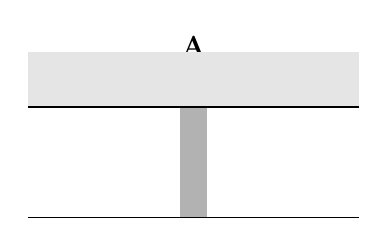
\begin{tikzpicture}[scale=0.7]
% A) Mafic dike in felsic host
\node at (0,1.1) {\textbf{A}};
\fill[gray!20] (-3,0) rectangle (3,1);
\fill[gray!60] (-0.25,0) -- (0.25,0) -- (0.25,-2) -- (-0.25,-2) -- cycle;
\draw (-3,0) -- (3,0); \draw (-3,-2) -- (3,-2);
\end{tikzpicture}

\vspace{1.2em}
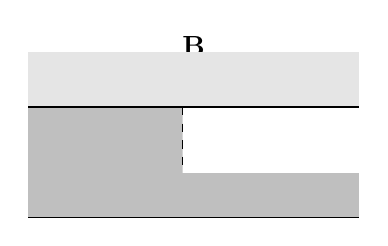
\begin{tikzpicture}[scale=0.7]
% B) Basement step + wedge
\node at (0,1.1) {\textbf{B}};
\fill[gray!20] (-3,0) rectangle (3,1);
\fill[gray!50] (-3,-2) -- (-3,0) -- (-0.2,0) -- (-0.2,-1.2) -- (3,-1.2) -- (3,-2) -- cycle;
\draw (-3,0) -- (3,0); \draw (-3,-2) -- (3,-2);
\draw[dashed] (-0.2,0) -- (-0.2,-1.2);
\end{tikzpicture}

\vspace{1.2em}
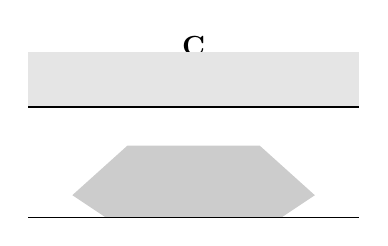
\begin{tikzpicture}[scale=0.7]
% C) Broad felsic pluton at depth
\node at (0,1.1) {\textbf{C}};
\fill[gray!20] (-3,0) rectangle (3,1);
\fill[gray!40] (-2.2,-1.6) -- (-1.2,-0.7) -- (1.2,-0.7) -- (2.2,-1.6) -- (1.6,-2) -- (-1.6,-2) -- cycle;
\draw (-3,0) -- (3,0); \draw (-3,-2) -- (3,-2);
\end{tikzpicture}
\end{center}

\columnbreak

\subsection*{Gravity Profiles (1--3)}
\begin{center}
% Profiles are schematic line plots
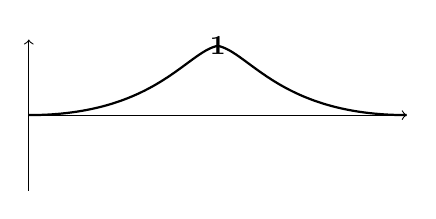
\begin{tikzpicture}[scale=0.8]
\node at (0,1.1) {\textbf{1}};
\draw[->] (-3,0) -- (3,0);
\draw[->] (-3,-1.2) -- (-3,1.2);
% narrow high-amplitude positive
\draw[thick] (-3,0) .. controls (-1,0) and (-0.5,1.0) .. (0,1.1)
                 .. controls (0.5,1.0) and (1,0) .. (3,0);
\end{tikzpicture}

\vspace{1.5em}
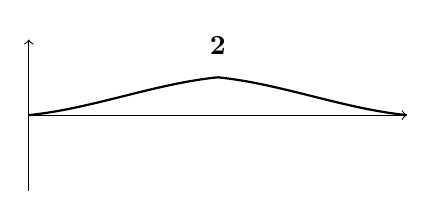
\begin{tikzpicture}[scale=0.8]
\node at (0,1.1) {\textbf{2}};
\draw[->] (-3,0) -- (3,0);
\draw[->] (-3,-1.2) -- (-3,1.2);
% broad gentle positive swell
\draw[thick] (-3,0) .. controls (-2,0.1) and (-1,0.5) .. (0,0.6)
                 .. controls (1,0.5) and (2,0.1) .. (3,0);
\end{tikzpicture}

\vspace{1.5em}
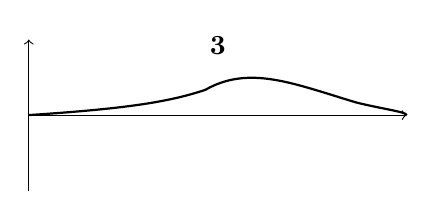
\begin{tikzpicture}[scale=0.8]
\node at (0,1.1) {\textbf{3}};
\draw[->] (-3,0) -- (3,0);
\draw[->] (-3,-1.2) -- (-3,1.2);
% asymmetric profile with shoulder
\draw[thick] (-3,0) .. controls (-1.5,0.1) and (-0.8,0.2) .. (-0.2,0.4)
                 .. controls (0.5,0.8) and (1.2,0.5) .. (2.2,0.2)
                 .. controls (2.6,0.1) and (3,0.05) .. (3,0);
\end{tikzpicture}
\end{center}
\end{multicols}

\vspace{0.5em}
\noindent\textbf{Your matches:}\quad A $\to$ \underline{\hspace{1.5cm}} \quad B $\to$ \underline{\hspace{1.5cm}} \quad C $\to$ \underline{\hspace{1.5cm}}\\[0.5em]
\textbf{Tie-breaker observation (and why):} \underline{\hspace{12cm}}

\end{document}